\documentclass{article}
\usepackage[T1]{fontenc}
\usepackage[latin1]{inputenc}
\usepackage[brazilian]{babel}


\title{Método dos Elementos Finitos aplicado � resolu\c{c}\~ao de problemas do Eletromagnetismo}
\author{Thiago de Sousa Goveia }
\date{19 de Fevereiro de 2017}

\usepackage{natbib}
\usepackage{graphicx, import}
\usepackage{amsmath}
\usepackage{svg}
\usepackage{natbib}
\usepackage{apalike}

\begin{document}
\maketitle

% !TeX spellcheck = <none>
\section{Problema de Valor de Contorno}


Um problema modelado por equações diferenciais parciais bem-posto, segundo as definições de Hadamard (1923), é aquele que 	apresenta a existência, unicidade e estabilidade de solução. Por estabilidade entende-se que uma pequena alteração no modelo leva à uma pequena alteração na solução \citep[p. 18]{moh}. Para que estas condições sejam satisfeitas, é necessário que o modelo matemático descreva adequadamente o fenômeno analisado e que as condições de contorno, ou condições iniciais, sejam bem estabelecidas. Assim sendo, um problema de valor 

Um problema de valor inicial, \textbf{PVI}, é aquela que contém as condições iniciais do fenômeno, as quais são impostas sobre a variável dependente e suas derivadas em um único instante de tempo $t_0$. Um problema de valor de contorno \textbf{PVC}, por sua vez, apresenta as condições em pontos distintos, como por exemplo em $x_i$ e $x_f$. \citep[p. 447]{boyce_diprima}. Os sistemas de equações \ref{eq:pvi} e \ref{eq:pvc} mostram respectivamente um problema de valor inicial e de contorno, ambos de segunda ordem.

\begin{equation}
	\label{eq:pvi}
	\begin{cases}
		y'' + p(t)y' + q(t)y = f(t) \\
		y(t_0) = y_0 \\
		y'(t_0) = y_0'
	\end{cases}
\end{equation}


\begin{equation}
	\label{eq:pvc}
	\begin{cases}
		y''(x) + p(x)y'(x) + q(x)y(x) = f(x) \\
		y(x_i) = \alpha \\
		y'(x_f) = \beta
	\end{cases}
\end{equation}

Geralmente os PVI são dados em função do tempo enquanto os PVC são dados em função do espaço. \citep[p. 447]{boyce_diprima}.

As condições estabelecidas sobre a variável dependente, são condições \textbf{essenciais} ou de \textbf{Dirichlet}, enquanto as que são estabelecidas sobre as derivadas da variável dependente são  conhecidas como \textbf{naturais} ou condições de \textbf{Neumann}.

Além das restrições de Dirichlet e Neumann, conforme mostra a tabela \ref{tab:cond}, existem restrições específicas do fenômeno modelado, como por exemplo, condições de radiação ou de impedência para problemas do eletromagnetismo. \citep[p. 20]{jin}. 


\begin{table}	
	\centering
	\begin{tabular}{|c|c|}	
		\hline
		\textbf{Condição} 
		& \textbf{Tipo} \\	
		\hline
		$y(x_k) = y_k $ 
		& Dirichlet \\
		\hline
		$y(x_k) = 0$
		& Dirichlet Homogênea\  \\
		\hline
		$y'(x_k) = y_k$
		& Neumann \\
		\hline
		$y'(x_k) = 0$
		& Neumann Homogênea\  \\
		\hline
	\end{tabular}
	\caption{Exemplos de condições de contorno}
	\label{tab:cond}
\end{table}


A solução analítica de um PVC pode ser obtida por meio da integração direta ou a partir da aplicação de técnicas como a separação de variáveis, expansão em séries ou pela transformada de Laplace. \citep[p. 31, 191, 239]{boyce_diprima} \citep[p. 59, 263, 355]{powers}.
No entanto, existem problemas da engenharia e da ciência que não são lineares ou apresentam  condições de contorno complexas, existência de interfaces e grande quatidades de detalhes.  Estas características fazem com que a resolução analítica de tais problemas seja impraticável, sendo necessário recorrer a métodos numéricos para se obter uma solução aproximada. \citep[p. 447]{boyce_diprima}  \citep[p.397]{powers}.



%\section{Método das diferenças finitas}

Como dito anteriormente, métodos numéricos são utilizados para aproximar soluções de equações diferenciais. O MDF tem como objetivo, discretizar o domínio do problema e substituir cada derivada da equação por um quociente-diferença adequado
\citep[p. 684]{burden_faires}.


Sendo o domínio $ \Omega $ unidimensional e contínuo, o mesmo pode ser discretizado particionando-se o intervalo $]a, b[$ em subintervalos iguais. Para isso, seleciona-se um conjunto de $N$ pontos igualmente espaçados entre $a$ e $b$, e dessa forma, $ N + 1 $ subintervalos são obtidos. O conjunto $\Omega \cup \Gamma$ pode então ser reprentado na como um conjunto de valores discretos $x_i$, como mostra a equação a seguir: 

\begin{equation}
  x_i = a + ih,  i = 0, 1, ... N+1
\end{equation}

O incremento $h$ corresponde ao comprimento de cada subintervalo e é dado por:

\begin{equation}
  h = \frac{b-a}{N+1}
\end{equation}

Nos pontos interiores $ x_i$  com $i = 1, 2. .... N $, isto é, dentro da borda $ \{a, b\} $ ou no domínio $\Omega$, a equação diferencial a ser aproximada é dada na primeira equação do sistema  \ref{eq:edo2}.
Deseja-se obter o valor de $ y(x_i) $ como uma média do valor de seus vizinhos $ y(x_i + h) $ e $ y(x_i - h) $. Esta abordagem é chamada de diferença centrada, uma vez que o ponto $ y(x_i) $ a ser obtido é o ponto central de uma vizinhança. 

A aproximação da derivada é feita por meio da expansão em série de Taylor truncada. Como a equação a ser aproximada é de ordem 2, a expansão deve ser feita até uma ordem superior a 2. No caso do exemplo apresentado, a expansão foi feita até a ordem 3 e a notação do grande $O$ foi utilizada para denotar o erro do truncamento.

\begin{equation}
    \label{eq:dfr}
    y(x_i + h) = y(x_i) + hy'(x_i) + \frac{h^{2}}{2}y''(x_i) + \frac{h^{3}}{6}y'''(x_i) + O(h^{4})
\end{equation}

\begin{equation}
    \label{eq:dfl}
    y(x_i - h) = y(x_i) - hy'(x_i) + \frac{h^{2}}{2}y''(x_i) - \frac{h^{3}}{6}y'''(x_i) + O(h^{4})
\end{equation}

As equações \ref{eq:dfr} e \ref{eq:dfl} são as expansões truncadas. A soma dessas equações fornece o valor da segunda derivada na forma de diferença centrada.

\begin{equation}
    \label{eq:difcent2}
    y''(x_i) = \frac{y(x_i + h) - 2y(x_i) +y(x_i - h) - O(h^{2})}{h^2}
\end{equation}

 De forma similar, para a derivada de primeira ordem, obtém-se

\begin{equation}
    \label{eq:difcent}
    y'(x_i) = \frac{y(x_i + h) - y(x_i - h) - O(h)}{2h}
\end{equation}

Simplificando a notação de forma que $y_{i+1} = y(x_i + h)$ e $y_{i-1} = y(x_i - h)$ o sistema dado em \ref{eq:edo2} pode ser representado em termos discretos por meio o sistema ~\ref{eq:edoDisc}. Como se trata de uma aproximação, as parcelas relativas ao erro foram desconsideradas.

\begin{equation}
	\label{eq:edoDisc}
	\begin{cases}
		  \frac{y_{i+1} - 2y +y_{i-1}}{h^2} = p(x_i) \frac{y_{i+1} - y_{i-1}}{2h} +q(x_i)y + r(x_i)\\
			y(a) = \alpha \\
			y'(b) = \beta \\
			 i = 0, 1, ... N+1
	\end{cases}
\end{equation}

Reorganizando a equação do modelo de ~\ref{eq:edoDisc} no formato apresentado pela equação ~\ref{eq:sistLin} a solução se torna computacionalmente trivial. Iterando os valores de i, o conjunto de equações lineares pode ser colocado na forma matricial, sendo a matriz dos coeficientes, uma matriz tridiagonal.

\begin{equation}
	\label{eq:sistLin}
	e_i y_{i-1} + c_i y_i + d_i y_{i +1} = r_i
\end{equation}

\begin{equation}
\begin{bmatrix}
    c_1 & d_1 	& 0 	& 0  & \dots 	& 0 \\
    e_2 & c_2 	& d_2 	& 0  & \ddots 	& 0 \\
    0 	& \ddots 	& \ddots 	& \ddots  	 & \ddots 	& 0 \\
    0 	& 0 	& 0 	& e_N  	 & c_N 	& d_N 
\end{bmatrix}
\begin{bmatrix}
    y_1\\ y_2\\ \vdots \\y_N
\end{bmatrix}
=
\begin{bmatrix}
    r_1\\ r_2\\ \vdots \\r_N
\end{bmatrix}
\end{equation}

A discretização obtida em  ~\ref{eq:edoDisc} pode ser expandido para $n$ dimensões. As equações \ref{eq:lap} e \ref{eq:lapDisc} mostram a equação de laplace em duas dimensões e a mesma equação discretizada pelo método das diferenças finitas centradas.

\begin{equation}
    \label{eq:lap}
    \Delta u = \frac{\partial^2 u}{\partial^2 x} + \frac{\partial^2 u}{\partial^2 y} = 0
\end{equation}

\begin{equation}
	\label{eq:lapDisc}
	\begin{cases}
		 \frac{u(x_{i+1}, y) - 2u(x, y) +u(x_{i-1}, y)}{h^2} +
		 \frac{u(x, y_{i+1}) - 2u(x, y) +u(x, y_{i-1} )}{h^2} = 0 \\
			 i = 0, 1, ... N+1
	\end{cases}
\end{equation}

\section{Introdução ao Método dos Elementos Finitos}

Segundo \citep[p. 19, 27]{jin}, o método dos elementos finitos (MEF) é uma técnica numérica que possibilita a aplicação das funções de interpolação, utilizadas na aproximação de PVC, sobre subdomínios do problema.

Já segundo \citep[p. 13]{reddy}, o MEF trata-se de um método no qual o domínio do problema é visto como uma coleção de subdomínios, chamados de elementos finitos, sobre os quais, a equação que modela o problema é aproximada por um método variacional ou de resíduos ponderados.



Como foi dito anteriormente, a resolução analítica de muitos problemas físicos se torna impraticável à medida em que a sua  complexidade aumenta. 
A fim de contornar esta dificuldade, estratégias numéricas para a discretização do domínio e aproximação da solução foram desenvolvidas por matemáticos, engenheiros e cientistas \citep[p. 1]{zien}. 

Dentre estas estratégias destacam-se o método das diferenças (MDF) finitas e o método dos elementos finitos (MEF), mostrados na figura \ref{fig:mdfFem}. O MDF consiste na discretização do domínio do problema por meio de uma grade de pontos e na aproximação de cada derivada da equação por um quociente-diferença adequado
\citep[p. 684]{burden_faires}. Embora este método seja útil em muitos casos, se torna difícil aplicá-lo em problemas com geometria irregular ou com condições de contorno não usuais. \citep[p. 4]{huebner}

\begin{figure}[!htb]
\centering
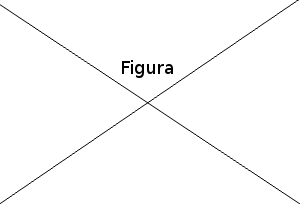
\includegraphics[scale=0.5]{figuras/temp.png}
\caption{Método das diferenças Finitas e método dos Elementos Finitos}
\label{fig:mdfFem}
\end{figure}

Diferentemente do MDF, como coloca \citep[p. 4]{huebner}, o MEF divide o domínio não em pontos, mas em subdomínios sobre os quais as equações são aproximadas por partes, e não pontualmente, como ocorre no MDF. O FEM também é capaz de representar mais fielmente o contorno (ou a borda) do problema. Desta forma, ele se apresenta como uma técnica mais poderosa e versátil para a modelagem de fenômenos com geometria complexa e meios não homogêneos \citep[p. 390]{sadiku}. 

O MEF surgiu originalmente como uma técnica de análise de deslocamentos e elasticidade de estruturas mecânicas, mas em seguida foi estendido para solucionar problemas de outros campos da física e da engenharia. \citep[p. 19]{jin} \citep[p. 3]{desai} \citep[p. 2]{zien}

As primeiras formulações do MEF são conhecidas como \textbf{abordagem direta} ou \textbf{formulação física}, que embora forneça a interpretação intuitiva do método, é util apenas para a resolução de problemas relativamente simples \citep[p. 6]{huebner}. O uso do princípio do trabalho virtual, para a determinação de forças na abordagem direta, levou à generalização do MEF, por meio da estratégia de minimização do funcional de energia. Esta técnica mais genérica  ficou conhecida como \textbf{formulação Variacional} \citep[p. 113]{desai} \citep[p. 20]{zien}. Uma terceira abordagem, conhecida como \textbf{Método dos Resíduos Ponderados} ou \textbf{MEF generalizado} \citep[p. 61]{zien} é tradicionalmente utilizada e é ainda mais genérica que o princípio Variacional, pois resolve diretamente as equações diferenciais do modelo, sem necessitar da existência de um funcional. \citep[p. 261]{desai}. Neste trabalho será adotado o método dos resíduos ponderados, mais especificamente, o método de Galerkin.


\subsection{Sistema de Elementos Discretos}
\citep[p. 68]{desai} introduz o conceito de Método de Elementos Discretos (MED) como sendo uma etapa intermediária da formulação física MEF. Na representação em elementos discretos, cada elemento é unidimensional, de tal forma que o sistema completo é representado por uma estrutura aramada, conforme mostra a figura \ref{fig:arame}.

De forma similar, \citep[p. 2]{zien} apresenta o Sistema Discreto Padrão (SDP) como uma forma unificada de analisar problemas de natureza discreta.

Em ambos os casos, os sistemas originais não se tratam de um contínuo, propriamente dito, mas de um sistema composto por partes, no entanto, são muito úteis na compreensão do funcionamento do MEF e do conceito de elemento.


\begin{figure}[!htb]
\centering
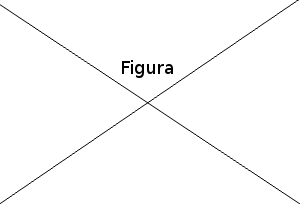
\includegraphics[scale=0.5]{figuras/temp.png}
\caption{Estruturas aramadas idealizadas}
\label{fig:arame}
\end{figure}





\subsection{Etapas de Processamento}
A computação de um problema modelado a partir de elementos finitos compreende basicamente três etapas: 
\begin{enumerate}  
\item \textbf{Pré-processamento}: Entrada de Dados ou discretização;
\item \textbf{Processamento}: Análise do problema e  solução do sistema de equações;
\item \textbf{Pós-processamento}: Apresentação dos Resultados. 
\end{enumerate}

Cada etapa apresenta uma contribuição para que se obtenha um resultado satisfatório. O pré-processamento é responsável pela discretização e por estabelecar as restrições físicas do domínio. A etapa de análise obtém a aproximação do modelo (forma fraca), e aplica esta aproximação em cada sub-domínio. O resultado preliminar da análise é um sistema de equações lineares que quando resolvido, fornece a solução do problema.  O pós-processamento consiste na exibição adequada dos resultados \citep[p. 665, 666]{zien}.


Nas seções a seguir cada etapa é vista em detalhes.

\section{Pré-Processamento}

A etapa de pré-processamento compreende a maior parte do tempo de modelagem do método. É neste ponto do processo que se são definidos os apectos geométricos do modelo, as propriedades dos materiais do objeto em análise e a aplicação das condições de contorno. \citep[p. 9, 665]{zien}

\subsection{Aspectos geométricos} 
A definição dos aspectos geométricos consiste na tranformação do domínio contínuo $\Omega$ em uma malha de elementos finitos. Cada elemento $\Omega_e$ dessa malha será tratado como um subdomínio de $\Omega,$.  
Nesta etapa são definidas a forma, o número e o tamanho dos elementos, de forma que a representação seja a mais próxima possível do objeto em análise \citep[p. 154]{desai}.
A figura \ref{fig:elementos} contém a representação de elementos tipicamente utilizados em 1, 2 e 3 dimensões. 

\begin{figure}[!htb]
\centering
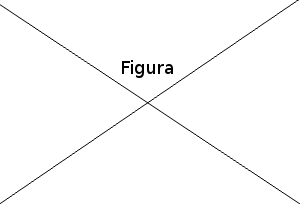
\includegraphics[scale=0.5]{figuras/temp.png}
\caption{Elementos em 1, 2 e 3 dimensões}
\label{fig:elementos}
\end{figure}

Conforme pode ser visto na figura \ref{fig:numeracao}, cada elemento pode ser identificado na malha a partir de um número que lhe é atribuído. De forma similar, os vértices (ou nós) também são numerados. Cada nó possui dois valores vinculados a ele. 
O primeiro número de cada par ordenado representa a numeração global nó, ou seja, a identificação do nó na malha. O segundo número do par ordenado é a numeração do nó dentro de um dado elemento (Identificação local). A numeração local é geralmente feita no sentido anti-horário, a fim de se obter um valor positivo no cálculo da área ou volume por meio do  determinante \citep[p. 394]{sadiku}. 

Um fator que deve ser levado em consideração é o balanceamento entre o refinamento da malha e o esforço computacional necessário \citep[p. 154]{desai}. Como o valor da solução é aproximado para cada elemento, o excesso de elementos pode causar a propagação do erro de aproximação, levando a resultados indesejáveis.


\begin{figure}[!htb]
\centering
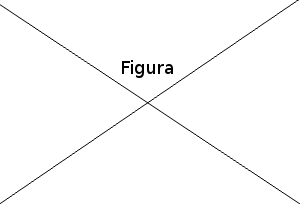
\includegraphics[scale=0.5]{figuras/temp.png}
\caption{Identificadores de Elementos e nós}
\label{fig:numeracao}
\end{figure}

\subsection{Propriedades do material}
Para que o MEF seja capaz de aproximar adequadamente a solução de um problema, é necessário, além da geometria, se especificar as propriedades do material de cada elemento da malha, sobretudo em meios não homogêneos. Na análise estrutural, por exemplo, aspectos como a plasticidade, elasticidade e porosidade podem afetar os resultados. \citep[p. 250]{desai}. Já na análise eletromagnética, algumas propriedades relevantes são a condutividade ($\sigma$), permeabilidade ($\mu$) e a permissividade ($\epsilon$) \citep[p. 3]{volakis}. Na análise térmica algumas propriedades importantes são o calor específico e a condutividade térmica \citep[p. 251]{desai}.
Desta forma, de acordo com a área de análise, os materiais apresentam características determinantes para a obtenção de resultados adequados.

As propriedades dos materiais podem ainda estar condicionadas à uma determinada direção. Desta forma, os materiais podem ainda ser classificados como isotrópicos ou anisotrópicos\citep[p. 20]{sadiku}.  Materiais isotrópicos apresentam as mesmas propriedades físicas em todas as direções. Nos materiais anisotrópicos, as propriedades variam conforme a direção considerada.

Fenômenos eletromagnéticos dependem adicionalmente da linearidade do meio. Meios lineares são aqueles em que a condutividade, a permeabilidade e a permissividade independem da intensidade do campo elétrico e do campo magnético \citep[p. 20]{sadiku} .


\subsection{Valores de Contorno}
A atribuição dos valores de contorno é o último passo da etapa de pré- processamento. Estes valores são atribuídos a pontos específicos da malha e são importantes para caracterizar a unicidade de solução. \citep[p. 7]{zien}

Considere um capacitor de placas paralelas, no qual uma das armaduras é submetida à uma tensão de 10V e outra à 0V. A ditribuição de potencial e o valor do campo elétrico entre as placas e no ambiente em volta do capacitor, podem ser definidos unicamente a partir das condições de contorno (10V e 0V) impostas em pontos (ou nós) específicos do domínio, como mostra a figura \ref{fig:capacitor}.

\begin{figure}[!htb]
\centering
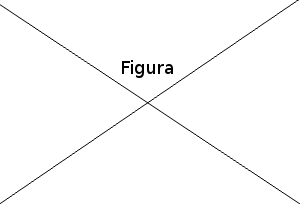
\includegraphics[scale=0.5]{figuras/temp.png}
\caption{Distribuição do potencial e o campo elétrico no capacitor de placas paralelas}
\label{fig:capacitor}
\end{figure}


\section{Processamento ou Análise de Elementos Finitos}
A etapa de processamento do MEF consiste basicamente em 3 passos \citep[p. 31]{jin}:

\begin{enumerate}  
\item Seleção das funções de interpolação;
\item Formulação do sistema de equações;
\item Solução do sistema de equações. 
\end{enumerate}

Cada um dos passos acima serão brevemente apresentados nesta seção, mas dada a sua importância e amplitude, eles serão aprofundados nas seções seguintes.

\subsection{Seleção das funções de interpolação}
O primeiro passo na etapa de processamento é a escolha de uma função de interpolação (função de base ou função de forma) \citep[p. 37]{volakis} que fornece uma aproximação da equação em cada elemento \citep[p. 32]{jin}. 
A função interpoladora escolhida geralmente é um polinômio, e isso ocorre por dois motivos a priori: \citep[p. 77]{desai}

\begin{itemize}  
\item Facilidade de manipulação matemática, principalmente derivação e integração;
\item Aproximação satisfatória quando truncado em uma ordem qualquer.
\end{itemize}

Na prática são escolhidos polinômios de primeira ou segunda ordem, mas ordens superiores podem ser adotadas para reduzir o erro de aproximação, no entanto, ocorre também o aumento da carga computacional \citep[p. 32]{jin}.

Sendo $N$ a função interpoladora, a solução aproximada $\tilde{\phi}$ para cada um dos $n$ nós de um dado elemento $e$ pode ser dada como:

 \begin{equation}
 	\label{eq:interpol}
		\tilde{\phi^e} = \sum_{j=1}^{n}{N_j^e \phi_j^e} = 
		\{N^e\}^T \{\phi^e\} = \{\phi^e\}^T \{N^e\}
 \end{equation}

Neste caso, $N_j^e$ é a função de forma do nó $j$ no elemento $e$ e $\phi_j^e$ é o valor de $\phi$ no nó $j$ do elemento $e$.
Uma característica importante a ser obervada nas funções $N_j^e$ é que elas são diferentes de zero apenas sobre o subdomínio $e$.

\subsection{Formulação do sistema de equações}
Métodos variacionais ou de resíduos ponderados são tradicionalmente utilizados para se obter um sistema de equações que satisfaça um modelo diferencial \citep[p. 34]{jin}. No modelo de elementos discretos apresentado anteriormente, o sistema de equações existe naturalmente.

Na abordagem variacional destaca-se o método de Ritz, ou Rayleigh-Ritz, o qual tem por objetivo, minimizar o funcional variacional, ou funcional de energia, do problema aproximado \citep[p. 24]{volakis}. Embora tal abordagem tenha sido historicamente utilizada e possua fundamentação física e matemática, sua adoção, em muitos casos, é mais complicada em relação ao Método dos Resíduos Ponderados, pois demanda a formulação variacional do problema. Desta forma, se um problema é dado por um modelo diferencial, é necessário se obter a partir deste modelo a forma variacional equivalente, para só então se aplicar o método para a obtenção do sistema de equações. No eletromagnetismo, a formulação variacional das equações de Maxwell não é bem estabelecida \citep[p. 211]{jin}.

Para problemas que apresentam explicitamente condições de Dirichlet no contorno e cujo operador $\mathcal{L}$ é linear e auto-adjunto, é possível se obter imediatamente o funcional (ou forma variacional) \citep[p. 81]{zien}, no entanto, como mostra \citep[p. 29]{volakis}, a mesma integral da formulação variacional é obtida pelo método de Galerkin.

\subsubsection{O método dos resíduos ponderados}

Seja a equação \ref{eq:operador}, uma equação diferencial que modela um determinado fenômeno físico, na qual $\mathcal{L}$ é um operador diferencial, $f$ é uma função de excitação conhecida e $\phi$ é a solução procurada \citep[p. 20]{jin}\citep[p. 24]{volakis}.

 \begin{equation}
 	\label{eq:operador}
	\mathcal{L} \phi = f
 \end{equation}
 
 Se substituirmos a solução exata pela sua aproximação apresentada na equação \ref{eq:interpol}, um resíduo $r$ surge, como pode ser visto na equação \ref{eq:residuos}, em decorrencia dos erros de aproximação.
 
  \begin{equation}
  	\label{eq:residuos}
 	r = \mathcal{L} \tilde{\phi} - f \neq 0
  \end{equation}

Como não se pode requerer que os resíduos da aproximação seja zero sobre todo o domíno $\Omega$ (o que ocorre na solução exata), faz-se a aproximação ou poderação dos resíduos em cada subdomínio $e$, como mostram as equações \ref{eq:res1} e \ref{eq:res2}. Desta forma, na média, a condição residual é atendida. \citep[p. 28]{volakis}

  \begin{equation}
  	\label{eq:res1}
 	R_i = \int_{\Omega}{w_i r \ d\Omega} = 0
  \end{equation}
  
  \begin{equation}
  	\label{eq:res2}
 	R_i = \int_{\Omega}{w_i [\mathcal{L} \tilde{\phi} - f] \ d\Omega} = 0
  \end{equation}  


A escolha particular de $w_i = \phi_i$ configura o método de Galerkin, o qual, para um operador $\mathcal{L}$ auto adjunto, fornece o mesmo resultado que o método de Ritz  \citep[p. 22]{jin}, conforme a seguinte equação

  \begin{equation}
  	\label{eq:galerkin}
 	R_i = 
 	\int_{\Omega}{N_i \mathcal{L} \{N\}^T \{\phi\} \ d\Omega\}} - \int_{\Omega}{N_i f \ d \Omega} = 0
  \end{equation}  
  
  
  o Resultado da equação \ref{eq:galerkin} é um sistema esparso de equações lineares, representado na equação \ref{eq:sistema}. Se o operador diferencial for auto-adjunto, o sistema é simétrico \citep[p. 36]{volakis}.
  
    \begin{equation}
    	\label{eq:sistema}
		[K]\{\phi\} = {b}
    \end{equation}  

É importante colocar que o parâmetro $w_i$ deve ser um conjunto de funções integraveis, linearmente independentes
\citep[p. 60]{reddy}. Alguns casos especiais do método dos resíduos ponderados são obtidos a partir da escolha de $w_i$:

\begin{equation}
\label{eq:metPond}
	\begin{tabular}{ l l }
	Método de Petrov-Galerkin & $ w_i = \psi_i \neq \phi_i $ \\ 
	Método de Galerkin & $ w_i = \phi_i $\\  
	Método dos Mínimos quadrados & $ w_i = \frac{d}{dx} \left(a(x)\frac{d \phi_i}{dx}\right) $ \\ 
	Método da colocação & $ \delta(x - x_i)  $ 
	\end{tabular}
\end{equation}



\paragraph{Funções sobre o espaço discreto \\}

Nesta seção será apresentada a visão geral do método. Para tal, os conceitos de formulação forte e fraca não serão necessários, visto que os problemas aqui descritos são modelados por sistemas lineares e não por equações diferenciais. Assim sendo, o MEF pode ser aplicado diretamente ao problema, sem a necessidade de se obter a forma integral (forma fraca) a partir de técnicas à relaxação da forma forte, como por exemplo o princípio dos trabalhos virtuais (abordagem direta), o método de Ritz (abordagem Variacional) e de Galerkin (abordagem por Resíduos ponderados).

Considere a malha bidimensional  apresentada na figura \ref{fig:malhaGenerica}. Esta malha pode representar por exemplo, a abstração de uma ponte metálica, de dutos de um fluido ou até mesmo um circuito elétrico, como apresentado na figura \ref{fig:repMalhaGenerica}.
\begin{figure}[!htb]
\centering
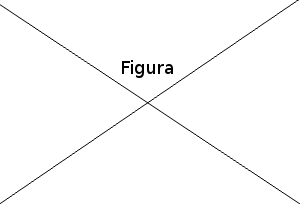
\includegraphics[scale=0.5]{figuras/temp.png}
\caption{Malha Genérica}
\label{fig:malhaGenerica}
\end{figure}

\begin{figure}[!htb]
\centering
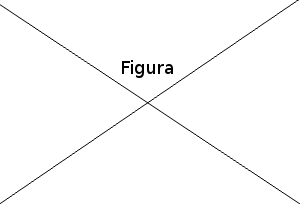
\includegraphics[scale=0.5]{figuras/temp.png}
\caption{Possíveis objetos de representação da malha \ref{fig:malhaGenerica}}
\label{fig:repMalhaGenerica}
\end{figure}


 Fazendo uma analogia com uma estrutura metálica, conforme apresentado na figura \ref{fig:repMalhaGenerica}-a, as forças que atuam nos nós, podem ser definidas  a a partir dos deslocamento destes nós, da distribuição da carga sobre um dado elemento e da tensão inicial, caso haja.
 
 Supondo que um carregamtno $p$ atue sobre o elemento $1$, as forças que atuam sobre os nós deste elemento podem ser dadas por:
 
 
 \begin{equation}
 	\label{eq:forca}
 	\begin{tabular}{c c}
 	$q_1 = 
		\left \{
 		\begin{tabular}{c}
	 		$q_1^1$ \\
	 		$q_2^1$ \\
	 		$q_3^1$
  		\end{tabular} 		
		\right \}$
		\
 	$q_1^1 = 
		\left \{
 		\begin{tabular}{c}
	 		$U_1$ \\
	 		$V_1$
  		\end{tabular} 		
		\right \}	$
		\end{tabular} 	
 \end{equation}


Similarmente, os deslocamentos podem ser dados para cada nó do elemento. Se as componentes da força na direção de x e y são dadas como U e V, as componentes da força podem ser dadas em função dessas componentes de deslocamento.

 \begin{equation}
 	\label{eq:desloc}
 	\begin{tabular}{c c}
 	$u_1 = 
		\left \{
 		\begin{tabular}{c}
	 		$u_1^1$ \\
	 		$u_2^1$ \\
	 		$u_3^1$
  		\end{tabular} 		
		\right \}$
		\
 	$u_1^1 = 
		\left \{
 		\begin{tabular}{c}
	 		$u_1(U_1)$ \\
	 		$v_1(V_1)$
  		\end{tabular} 		
		\right \}	$
		\end{tabular} 	
 \end{equation}


Assumindo um material isotrópico, cujo comportamento é linear elástico, a lei de Hooke fornece a equação \ref{eq:hooke}

 \begin{equation}
 	\label{eq:hooke}
	\textbf{$q^1 = K^1 u^1 + f^1$}
 \end{equation}
 
 O vetor $q$ representa as forças induzidas pelos deslocamentos $u$ dos nós. A matriz $K$ é a matriz de rigidez ou matriz de coeficientes do problema. $f$ é a força ou tensão inicial do elemento. Caso o estado inicial do elemento seja de equilíbrio, $f$ é igual a zero.
 
 Para que a representação seja adequada é necessário que sejam estabelecidas condições de compatibilidade de deslocamentos e equilíbrio.
 
 A compatibilidade de deslocamento é necessária, uma vez que quando um nó de um elemento é deslocado em uma direção, os elementos vizinhos que compartilham o mesmo nó também são afetados com este deslocamento. Esta condição é satisfeita aos se relacionar todas as forças do sistema.
 
 \paragraph{Montagem do Sistema Global}
 
 Para que o conjunto de funções de força ou tensão sobre os subdomínios sejam corretamente agregadas em um sistema global, é necessário se estabelecer as condições de compatibilidade de deslocamento e de equilíbrio.
 
 Como um nó de um elemento é compartilhado com os elementos vizinhos, a compatibilidade dos deslocamentos ocorre por meio da montagem de um sistema global. Este sistema possibilita que todos os deslocamentos estejam relacionados entre si.
 
  A figura \ref{fig:loc2glob} mostra a transformação dos sistemas locais para um sistema com referências globais. Como todos os nós são relacionados entre si, a matriz de rigidez é quadrada e também simétrica para o caso de materiais isotrópicos.
  
  \begin{figure}[!htb]
  \centering
  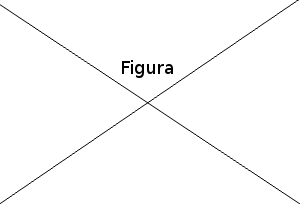
\includegraphics[scale=0.5]{figuras/temp.png}
  \caption{}
  \label{fig:loc2glob}
  \end{figure}
  
  O sistema em \ref{eq:assembly} mostra a relação entre todos os pontos do domínio para um dado elemento. é importante notar que apenas elementos adjacentes se afetam mutuamente.
  
 \begin{equation}
 	\label{eq:assembly}
 	\begin{tabular}{c c c}
 	$q^e = 
		\left \{
 		\begin{tabular}{c}
	 		$q^e_1$ \\
	 		$q^e_2$ \\
	 		\vdots \\
	 		$q^e_m$
  		\end{tabular} 		
		\right \}$
		\
 	$u^e = 
		\left \{
 		\begin{tabular}{c}
	 		$u_1$ \\
	 		$u_2$ \\
	 		\vdots \\
	 		$u_m$
  		\end{tabular} 		
		\right \}	$
		\
		$K^e =
		\begin{bmatrix}
		    K^e_{11} 	& K^e_{12}  & \dots 	& K^e_{1m} \\
		    K^e_{11} 	& \ddots  & \ 	& \vdots \\
		    \vdots 	& \vdots  	 & \ 	& \vdots \\
		    K^e_{m1} 	& \dots   & \dots 	& K^e_{mm} 
		\end{bmatrix}	 $		
	\end{tabular} 
 \end{equation}
 
 Com os deslocamento relacionados em todos os pontos elementos do sistema,
 a condição de equilíbrio é satisfeita quando o somatório das forças causadoras de tais deslocamentos nula, ou seja, a resultante em um dado ponto $a$ vale zero.
 
  \begin{equation}
  	\label{eq:somaForcas}
 	\sum_{e=1}^{m}{q_a^e = q_a^1 + q_a^2 + \dots = 0}
  \end{equation}
  
  Considerando que o corpo está inicialmente em equilíbrio, ou seja, $f = 0$, o sistema como um todo pode ser representado como 
  
    \begin{equation}
    	\label{eq:equilibrio}
    	q =
   		\sum_{b=1}^{n}\sum_{e=1}^{m}{K_{ab}^e u_b = 0}
    \end{equation}
    
    
\paragraph{Atribuição das condições de Contorno \\}
A atribuição dos valores de contorno da variável $u$ consiste na especificação dos deslocamentos ou deformações prefixadas no sistema. No exemplo \ref{fig:repMalhaGenerica}-a, como análise estrutural, as condições de contorno podem ser os deslocamentos nulos impostos nós fixados (soldados) ou condições iniciais de tensão ou torção. a equação \ref{eq:condIni} exemplifica a atribuição dessas condições.

\begin{equation}
   	\label{eq:condIni}
 	u_1 = u_6 = 
		\left \{
 		\begin{tabular}{c}
	 		$0$ \\
	 		$0$ \\
  		\end{tabular} 		
		\right \}	
\end{equation}

A inserção de valores de contorno no sistema promove a redução do número de equações de equilíbrio, por meio da eliminação das linhas cujo valor de $u$ já foi especificado.

\paragraph{Exemplo \\}

A fim de exemplificar a etapa de processamento,  considere a malha de resistores introduzidas  em \ref{fig:repMalhaGenerica}-b. Neste caso, as condições de contorno são as a tensões fornecidas por uma bateria.

\subsubsection{Pós-Processamento}
A etapa de pós processamento consiste na apresentação dos resultados obtidos no processamento e na determinação de variáveis secundárias a partir destes resultados.

A apresentação da solução pode ser feita graficamente por diferentes técnicas, como curvas de nível, mapas vetoriais, sobreposição de imagens e animações. Alguns exemplos são dados na figura \ref{fig:graf}

\begin{figure}[!htb]
\centering
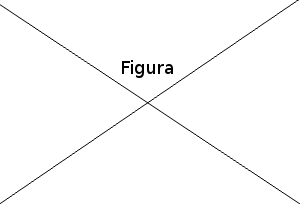
\includegraphics[scale=0.5]{figuras/temp.png}
\caption{}
\label{fig:graf}
\end{figure}

Com base nos valores apresentados no pós processamento, novas decisões são tomadas, tanto para otimizar os resultados quanto para melhorar a performance.

\subsection{Abordagem Direta \\}

A abordagem direta, abordagem física ou formulação de deslocamentos foi a primeira tentativa de se modelar um problema físico em termos de elementos finitos.

Voltada para a análise de estruturas e problemas de elasticidade, esta técnica busca aproximar o comportamento de um problema contínuo, por meio de elementos finitos, que se comporte de maneira similar a elementos reais discretos.
\citep[p. 19]{zien}

A partir desta abordagem, a forma fraca do problema diferencial é obtida com o uso do princípio dos trabalhos virtuais.
\citep[p. 20]{zien}

 


\subsection{Método Variacional}
Os métodos variacionais são técnicas utilizadas para extremizar o valor de um funcional em um determinado espaço de funções. Por extremizar entende-se encontrar o valor mínimo, máximo ou o ponto de inflexão do funcional.
Sistemas físicos, segundo o princípio de Hamilton ou princípio da mínima ação, tendem a minimizar sua energia interna ao realizar trabalho. Dessa forma, problemas envolvendo modelos matemáticos podem ser resolvidos considerando-se o problema de minimização de energia equivalente. (\textbf{Nota:} Um apêndice sobre elasticidade plana, princípio de Hamilton e análise funcional deve ser acrescentado).

Um funcional $ I(y) $ é uma regra que associa cada função $ u $ de um domínio $ \Omega $ a um único número real:

\begin{equation}
I : y \rightarrow \Re
\end{equation}

Em linhas gerais, pode ser entendido como uma função de funções. Um exemplo típico de funcional é a integral definida a seguir, a qual mapeia a função $ y $ em um valor real.

\begin{equation}
\label{eq:funcional}
I = \int_{a}^{b} u(y, y', x) dx
\end{equation}

Se uma função $ y(x) $ , por exemplo, minimiza o funcional, qualquer variação infinitesimal $ \alpha $ em $ y(x) $ produzirá um valor maior no funcional $ I $, o qual deixará de satisfazer a condição de mínimo. O operador variacional $ \delta $ desloca a função $ y $ em uma distância igual a $ \alpha \eta(x) $, sendo $ \alpha $ uma constante que tende a zero e $ \eta $ uma função suave definida em $[a,b]$, tal que $\eta(a) = \eta(b) = 0$.

Assim, tem-se: 

\begin{equation}
	\label{eq:sisEta}
	\begin{cases}
        y(x, \alpha) = y(x) + \alpha \eta(x) \\
        y(x, \alpha)' = y(x)' + \alpha \eta'(x) \\
		\alpha \eta(x) = \delta y(x) \\   
		\alpha \eta'(x) = \delta y'(x) \\  
    \end{cases}
\end{equation}

Se substituirmos as equações de \ref{eq:sisEta} em \ref{eq:funcional} o valor do funcional passa depender tanto da função $ y $ quanto de suas variações, realizadas pelo parâmetro $ \alpha $.

\begin{equation}
\label{eq:funcionalVar}
I(\alpha) = \int_{a}^{b} u(y(x, \alpha), y'(x, \alpha), x) dx
\end{equation}

A variação do funcional $ I $, pode ser entendida em termos diferenciais, como a derivada do funcional em relação ao incremento $\alpha$ da variação.

\begin{equation}
\delta I = \frac{\partial I}{\partial \alpha}
\end{equation}

O valor extremo procurado (mínimo, máximo ou ponto de inflexão) é caracterizado por possuir a primeira derivada igual a zero, portanto:

\begin{equation}
\delta I = \frac{\partial}{\partial \alpha} \int_{a}^{b} u(y(x, \alpha), y'(x, \alpha), x) dx = 0
\end{equation}

\begin{equation}
\delta I = \int_{a}^{b} \left(\frac{\partial u}{\partial y} \frac{\partial y}{\partial \alpha} + \frac{\partial u}{\partial y'} \frac{\partial y'}{\partial \alpha}\right) dx = 0
\end{equation}

Das equações em \ref{eq:sisEta} tem-se 

\begin{equation}
\begin{split}
\delta I = \int_{a}^{b} \left(\frac{\partial u}{\partial y} \eta + \frac{\partial u}{\partial y'} \frac{\partial }{\partial x}
\frac{\partial y}{\partial \alpha}\right) dx \\
= \int_{a}^{b} \left(\frac{\partial u}{\partial y} \eta + \frac{\partial u}{\partial y'} \eta'
\right) dx = 0
\end{split}
\end{equation}

É importante notar que a variação ocorre apenas no conjunto imagem do funcional, assim $\frac{\partial{x}}{\partial{\alpha}} = 0$. Integrando separadamente o segundo termo por partes tem-se:

\begin{equation}
\begin{split}
\delta I = \int_{a}^{b} \eta \left(\frac{\partial u}{\partial y} - \frac{d}{dx} 
\frac{\partial u}{\partial y'}\right)  dx +
\left[\frac{\partial u}{\partial y'} \eta(x) \right]_a^b
\end{split}
\end{equation}

Uma vez que a variação no contorno é zero (fronteiras fixas), $\eta(a) = \eta(b) = 0$, o valor de $ \delta I $ é dado por:

\begin{equation}
\label{eq:intEuler}
\begin{split}
\delta I = \int_{a}^{b} \eta \left(\frac{\partial u}{\partial y} - \frac{d}{dx} 
\frac{\partial u}{\partial y'}\right)  dx = 0
\end{split}
\end{equation}

Sendo $ \eta $ uma função derivável em $ [a,b] $, para que a igualdade \ref{eq:intEuler} seja satisfeita, torna-se necessário que o termo entre parentesis seja igual a zero

\begin{equation}
\label{eq:euler}
\frac{\partial u}{\partial y} - \frac{d}{dx} 
\frac{\partial u}{\partial y'} = 0, \ a < x < b
\end{equation}

Do conjunto de funções admissíveis, a única função que minimiza o funcional $I$  e portanto a energia interna do processo físico, é a mesma que resolve a equação \ref{eq:euler}, conhecida como Equação de Euler-Lagrange.

\subsection{Método dos Resíduos ponderados}

O método dos elementos finitos consiste em encontrar uma  solução do problema diferencial por meio da aproximação por polinômios 
\citep[p. 97]{davis}. Uma vez que aproximações geram erros, aqui chamados de resíduos, torna-se necessário reduzir tais resíduos para que se tenha uma aproximação de qualidade.

Uma vez que o método opera sobre um domínio $ \Omega $ discreto, tal que $ \Omega \approx \sum \Omega_j $,  os polinômios utilizados na aproximação são definidos por partes no domínio $\Omega$, isto é, são diferentes em apenas um intervalo do domínio.

O somatótrio definido na equação \ref{eq:pppol} aproximação da solução $ u $ de uma equação diferencial. As contantes $ c_j $ são os coeficientes desconhecidos e as funções $ \phi_j $, chamadas de funções de forma, são conhecidas, diferenciaveis por partes no domínio $ \Omega $ e de respeitam as condições de contorno, ou seja $ \phi_j(a) = \phi_j(b) = 0 $. 
 

\begin{equation}
	\label{eq:pppol}
	u(x) \approx U_N (x) = \sum_{j = 1}^{N} c_j \phi_j (x)
\end{equation}

Considere a forma geral da equação diferencial a ser resolvida, indicada pelo operador diferencial $ \mathcal{L} $:
 
 \begin{equation}
 	\label{eq:opDif}
 	\mathcal{L} u = f
 \end{equation}
 
 Uma vez que $U_N$ é um resultado aproximado de $u$, mas não necessariamente igual, a desigualdade a seguir é válida e conhecida como \textbf{residual da aproximação}.
 
 \begin{equation}
 \label{eq:residuo}
 	R(x, c_j) = \mathcal{L} U_N - f \neq 0
 \end{equation}
 
 De modo a obter a aproximação mais adequada, deve-se minimizar o resíduo da aproximação em todo o domínio. Uma vez que não se pode requerer que os resíduos de todos os subdomínios sejam zero, como mostrado na equação ~\ref{eq:residuo}, faz-se a ponderação dos mesmos por meio de funções $w$ de forma a atender a condição residual dada a seguir:
 \begin{equation}
 \label{eq:intResPond}
	\int_{\Omega} w_i(x)R(x, c_i)d\Omega = 0, \ i = (1, 2, ..., N)
 \end{equation} 
 
O parâmetro $w_i$ é um conjunto de funções integraveis linearmente independentes, chamadas de funções peso
\citep[p. 60]{reddy}.

Alguns casos especiais do método dos resíduos ponderados são obtidos a partir da escolha do parâmetro $w_i$ 

\begin{equation}
\label{eq:resPond}
	\begin{tabular}{ l l }
	Método de Petrov-Galerkin & $ w_i = \psi_i \neq \phi_i $ \\ 
	Método de Galerkin & $ w_i = \phi_i $\\  
	Método dos Mínimos quadrados & $ w_i = \frac{d}{dx} \left(a(x)\frac{d \phi_i}{dx}\right) $ \\ 
	Método da colocação & $ \delta(x - x_i)  $    ($\delta$ de Dirac)
	\end{tabular}
\end{equation}

\subsection{Formulação fraca do Problema}

A forma fraca, ou forma variacional de uma equação diferencial é uma integral ponderada, equivalente à equação diferencial e às suas condições naturais de contorno. Por meio da forma fraca obtem-se um conjunto de equações algébricas relacionadas aos coeficientes desconhecidos ($c_i$). Para diferentes escolhas da função de peso, diferentes equações algébricas serão obtidas.
\citep[p. 64]{reddy}

A obtenção da forma fraca será ilustrada com a equação diferencial a seguir e suas condições de contorno:

\begin{equation}
	\label{eq:exFFraca}
	\mathcal{L}u = \frac{d^2 u}{dx^2} = f, \ u(a) = \alpha, \ u(b) = \beta
\end{equation}

Antes de se aplicar a discretização (ou interpolação) dada em \ref{eq:pppol}, substitui-se o problema contínuo a ser resolvido, na integral dos resíduos ponderados:

\begin{equation}
	R = \frac{d^2 u}{dx^2} - f = 0
\end{equation}

 \begin{equation}
	\int_{a}^{b} w\left(\frac{d^2 u}{dx^2} - f\right) dx = 0
 \end{equation} 
 
 Integrando por partes:
 
 \begin{equation}
 \label{eq:fFracaG}
 \left.w \frac{du}{dx}\right|_{a}^{b} - 
	\int_{a}^{b} 
	\frac{du}{dx} \frac{dw}{dx} dx = \int_{a}^{b} wf dx
 \end{equation} 

A equação \ref{eq:fFracaG} é denominada forma fraca da equação \ref{eq:exFFraca}. Adicionalmente, verifica-se a condição de contorno. Se for considerado que $ w(a) = w(b) = 0$ por exemplo, tem-se:

 \begin{equation}
 - 	\int_{a}^{b} 
	\frac{du}{dx} \frac{dw}{dx} dx = \int_{a}^{b} wf dx
 \end{equation} 
 
 Substituindo a função contínua $u$ por sua aproximação $U_N$ e considerando o método de Galerkin:
 
  \begin{equation}
  - \int_{a}^{b} 
 	\frac{d}{dx} 
 	\sum_{j = 1}^{N} c_j \phi_j
 	\frac{d}{dx} \phi_i dx = \int_{a}^{b} f\phi_i dx, \ i = (1, 2, ..., N)
  \end{equation} 
  
    \begin{equation}
    -\sum_{j = 1}^{N} \int_{a}^{b} 
   	\frac{d c_j \phi_j}{dx}    	 
   	\frac{d \phi_i}{dx}  dx = \int_{a}^{b} f\phi_i dx, \ i = (1, 2, ..., N)
    \end{equation} 
    
    \begin{equation}
    \label{eq:matFraca}
    \sum_{j = 1}^{N} 
    	A_{ij} c_j = F_i,  \ i = (1, 2, ..., N)
    \end{equation} 
    
A equação  ~\ref{eq:matFraca} é a forma matricial obtida com a aplicação do método de Galerkin, a qual é esparsa e simétrica.

\section{Introdução ao Eletromagnetismo}

\subsection{Campos Eletrostáticos}

\subsection{Equações de Poisson e Laplace}

\subsection{Exemplo: Capacitor de placas paralelas}
\section{Conclusão Parcial}
Este relatório parcial abordou a resolução de PVC por meio de métodos numéricos. Fica como encargo dos próximos relatórios:

\begin{enumerate}
\item Formalizar os métodos de aproximação (Ritz, Petrov-Galerkin...);
\item Incluir exemplos com desenvolvimento mais detalhados;
\item Criar apêndices de demonstração e rigor matemático;
\item Aprofundar abordagem do MEF e fazer considerações estruturais;
\item Incluir todas as referências e formatar as citações;
\item Incluir imagens png/svg;
\item Iniciar a abordagem da teoria eletromagnética.
\end{enumerate}



\bibliographystyle{apalike}
\bibliography{references}
\end{document}
